\section{Results and Discussion}

\section{Standard Evolutionary Experiments}

\begin{figure*}%[!htbp]

\begin{center}
\setlength\tabcolsep{1.5pt} % default value: 6pt
\begin{tabular}{ | c || c c c | c c c | c | c | }
  \multicolumn{8}{c}{} & \multicolumn{1}{c}{Control} \\
  \multicolumn{1}{c}{} & \multicolumn{3}{c}{Competitors} & \multicolumn{3}{c}{Mean Dominant ($\pm S.D.$)} & \multicolumn{1}{c}{ Pop Mean ($\pm S.D.$)} & \multicolumn{1}{c}{ Pop Mean ($\pm S.D.$)} \\
 \cline{2-9}
  \multicolumn{1}{c|}{} & \tiny{$P_{1} = 1.0$} & \tiny{$P_{2} = P_{1}$} & \tiny{$P_{2} > P_{1}$} & \tiny{$P_{1} = 1.0$} & \tiny{$1.0 > P_{1} > P_{2}$} & \tiny{$P_{2} \geq P_{1}$} & \tiny{\textit{all}} & \tiny{\textit{all}}  \\
 \hline
 $Upd.$ & 25M & 25M & 25M & 25M & 25M & 25M & 200k & 200k \\
 $n$ & 1 & 1 & 1 & 9 & 7 & 34 & 50 & 50 \\
 \hhline{|=||===|===|=|=|}
 $A_1$ & 0.00 & 0.00 & 0.89 & $0.23 \pm 0.35$ & $0.50 \pm 0.47$ & $0.57 \pm 0.46$ & $0.51 \pm 0.14$ & $0.46 \pm 0.30$\\
 $A_2$ & 1.00 & 1.00 & 1.00 & $1.00 \pm  0.00$ & $1.00 \pm 0.00$ & $1.00 \pm 0.00$ & $1.00 \pm 0.00$ & $1.00 \pm 0.00$ \\
 \hline
 $P_{c}$ & 0.00 & 0.00 & 0.00 & $0.00 \pm 0.00$ & $0.00 \pm 0.00$ & $0.03 \pm 0.05$ & $0.07 \pm 0.03$ & $0.00 \pm 0.00$ \\
 $P_1$ & 1.00 & 0.50 & 0.00 & $1.00 \pm 0.00$ & $0.60 \pm 0.07$ & $0.28 \pm 0.16$ & $0.39 \pm 0.11$ & $0.04 \pm 0.08$ \\
 $P_2$ & 0.00 & 0.50 & 1.00 & $0.00 \pm 0.00$ & $0.40 \pm 007$ & $0.69 \pm 0.14$ & $0.54 \pm 0.11$ & $0.96 \pm 0.08$ \\
 \hline
 $C_1$ & 3.13 & 3.45 & 2.04 & $3.90 \pm 0.60$ & $3.38 \pm 0.33$ & $3.03 \pm 0.69$ & $3.38 \pm 0.23$ & $8.21 \pm 5.45$ \\
 $C_2$ & 233.2 & 238.6 & 290.2 & $230.6 \pm 71.1$ & $192.7 \pm 45.3$ & $271.6 \pm 73.6 $ & 99$.2 \pm 7.4 $& 350$.0 \pm 92.1 $ \\
 \hline
 $E_{c}$ & 0.87 & 0.14 & 4.20 & $0.29 \pm 0.37$ & $0.44 \pm 0.59$ & $0.21 \pm 0.75$ & $1.43 \pm 0.38$ & $2.77 \pm 1.50$ \\
 $E_1$ & 33.4 & 11.7 & 4.80 & $47.2 \pm 21.7$ & $21.3 \pm 12.0$ & $4.62 \pm 7.05$ & $31.5 \pm 6.6$ & $6.72 \pm 9.58$ \\
 $E_2$ & 341.4 & 397.4 & 321.1 & $231.2 \pm 94.3$ & $283.1 \pm 57.0$ & $325.4 \pm 68.9$ & $240.0 \pm 30.0$ & $317.5 \pm 55.2$ \\
 \hline
 $M_{c}$ & 0.11 & 1.00 & 0.66 & $0.33 \pm 0.41$ & $0.74 \pm 0.31$ & $0.67 \pm 0.35$ & $0.50 \pm 0.11$ & $0.20 \pm 0.23$ \\
 $M_1$ & 0.00 & 1.00 & 0.40 & $0.52 \pm 0.41$ & $0.65 \pm 0.46$ & $0.68 \pm 0.38$ & $0.50 \pm 0.12$ & $0.50 \pm 0.34$ \\
 $M_2$ & 0.00 & 0.44 & 1.00 & $0.45 \pm 0.39$ & $0.52 \pm 0.37$ & $0.50 \pm 0.42$ & $0.50 \pm 0.13$ & $0.50 \pm 0.33$ \\
 \hline
 $S_1$ & 0.00 & 1.00 & 1.00 & $0.65 \pm 0.38$ & $0.55 \pm 0.40$ & $0.47 \pm 0.42$ & $0.48 \pm 0.11$ & $0.48 \pm 0.34$ \\
 $S_2$ & 0.00 & 0.01 & 0.46 & $0.51 \pm 0.43$ & $0.35 \pm 0.39$ & $0.45 \pm 0.39$ & $0.49 \pm 0.13$ & $0.44 \pm 0.31$ \\
 \hline
\end{tabular}
\end{center}
\caption{
Enumerations for genotypes used as seeds for competition experiments (left) and enumerations for mean values of the most abundant genotype at the end of evolutionary runs (right), both sorted by resource-caching strategy.
}
\label{fig:genotypes}
\end{figure*}


\begin{figure*}%[!htbp]
\begin{center}
\thinmuskip=-2mu
\thickmuskip=-2mu
\nulldelimiterspace=-1pt
\scriptspace=0pt
\begin{subfigure}[b]{0.66\columnwidth}
  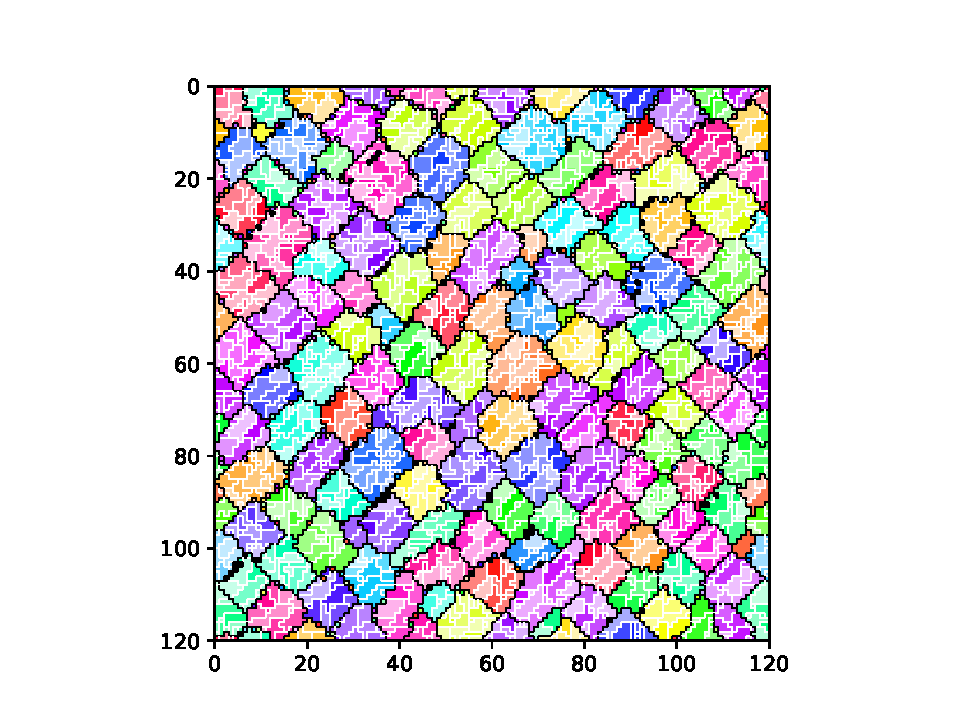
\includegraphics[width=\columnwidth,trim={2.5cm 0.5cm 2.5cm 1cm},clip]{img/ChannelMap_1022_update19500000}
  \caption{Mean $P_{c} = 0.77$, $P_1 = 0.09$, $P_2 = 0.14$; gen. 20,475}
  \label{fig:ChannelMap_1022}
\end{subfigure}%
\begin{subfigure}[b]{0.66\columnwidth}
  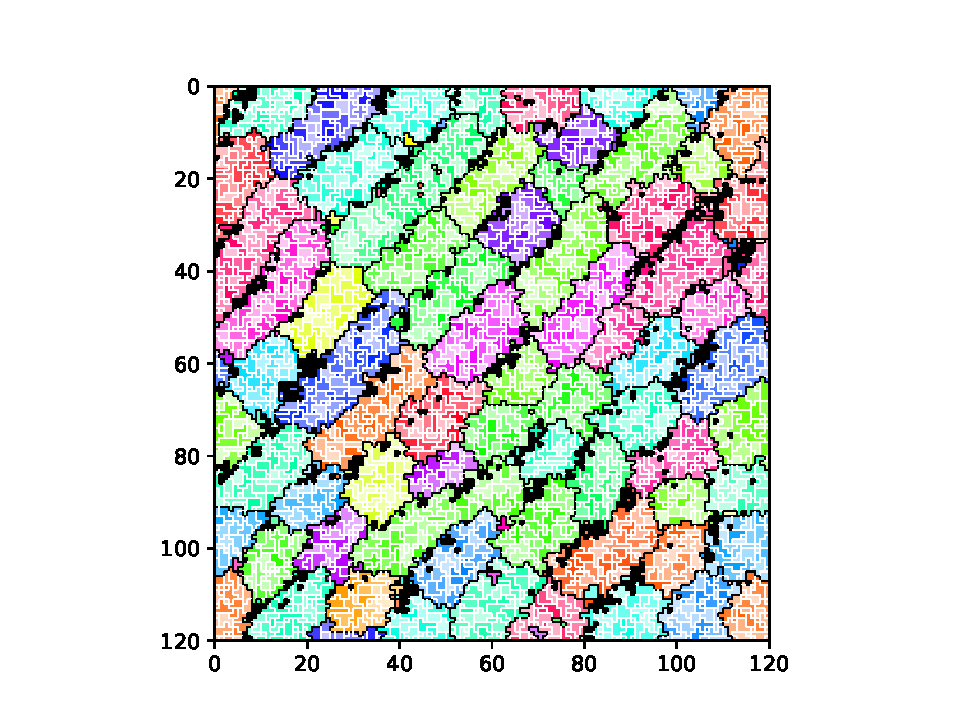
\includegraphics[width=\columnwidth,trim={2.5cm 0.5cm 2.5cm 1cm},clip]{img/ChannelMap_1041_update19500000}
  \caption{Mean $P_1 = 1.0$; gen. 23,971\\~}
  \label{fig:ChannelMap_1041}
\end{subfigure}%
\begin{subfigure}[b]{0.66\columnwidth}
  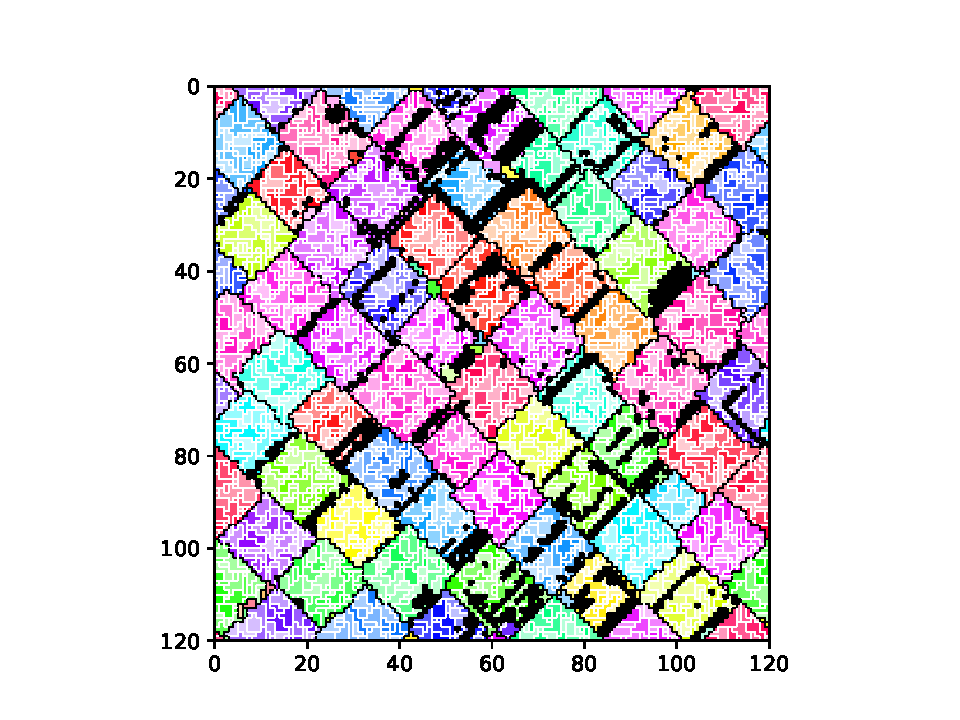
\includegraphics[width=\columnwidth,trim={2.5cm 0.5cm 2.5cm 1cm},clip]{img/ChannelMap_1008_update19500000}
  \caption{Mean $P_2 = 1.0$; gen. 25,841\\~}
  \label{fig:ChannelMap_1008}
\end{subfigure}

\caption{
End state of same-channel signaling networks in replicates where cell- (\ref{fig:ChannelMap_1022}), first- (\ref{fig:ChannelMap_1041}), and second-level (\ref{fig:ChannelMap_1008}) individuality dominated.
(Cell-level individuals are single cells that retain collected resource exclusively for their own use, first-level individuals are level-one same-channel multi-cellular networks that primarily assign collected resource for collective use among level-one channel mates, and second-level individuals are level-two same-channel multi-cellular networks that primarily assign collected resource for collective use among level-two channel mates.)
Level-one channels are coded by color saturation and level-two channels are coded by color hue.
A single cell-like organism occupies each grid tile except for black tiles, which are empty.
}
\label{fig:outcome_grids}
\end{center}
\end{figure*}


\begin{figure*}%[!htbp]
\begin{center}

\begin{subfigure}[b]{0.33\columnwidth}
  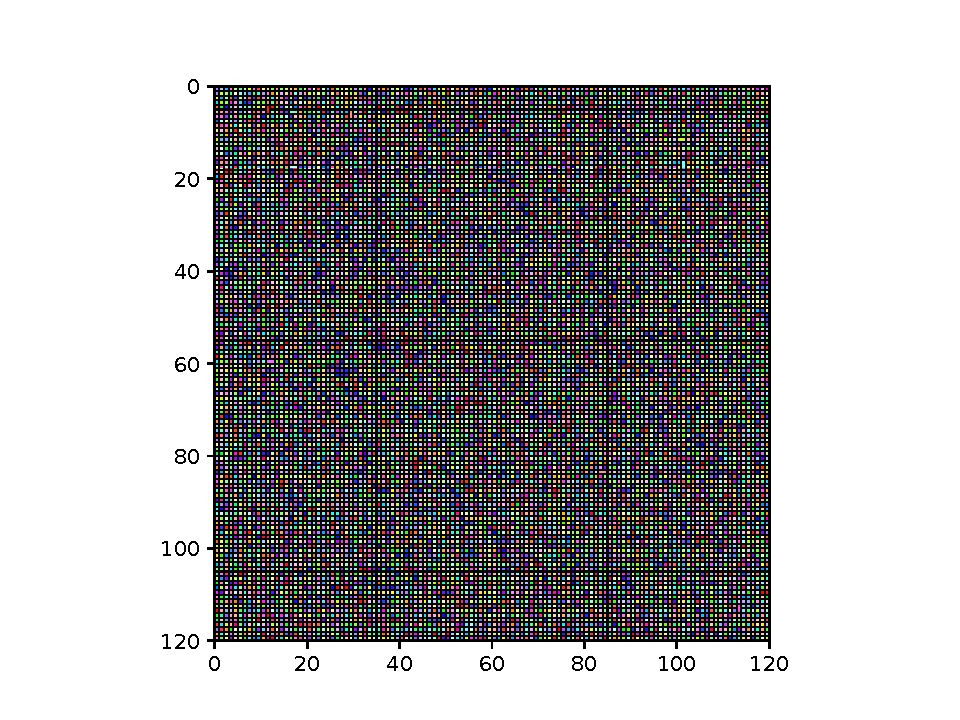
\includegraphics[width=\columnwidth,trim={2.5cm 0.5cm 2.5cm 1cm},clip]{img/ChannelMap_1007_update0}
  \vspace{-5ex}
  \caption{Update 0; cell gen. 0}
  \label{fig:ChannelMap_1007_update0}
\end{subfigure}%
\begin{subfigure}[b]{0.33\columnwidth}
  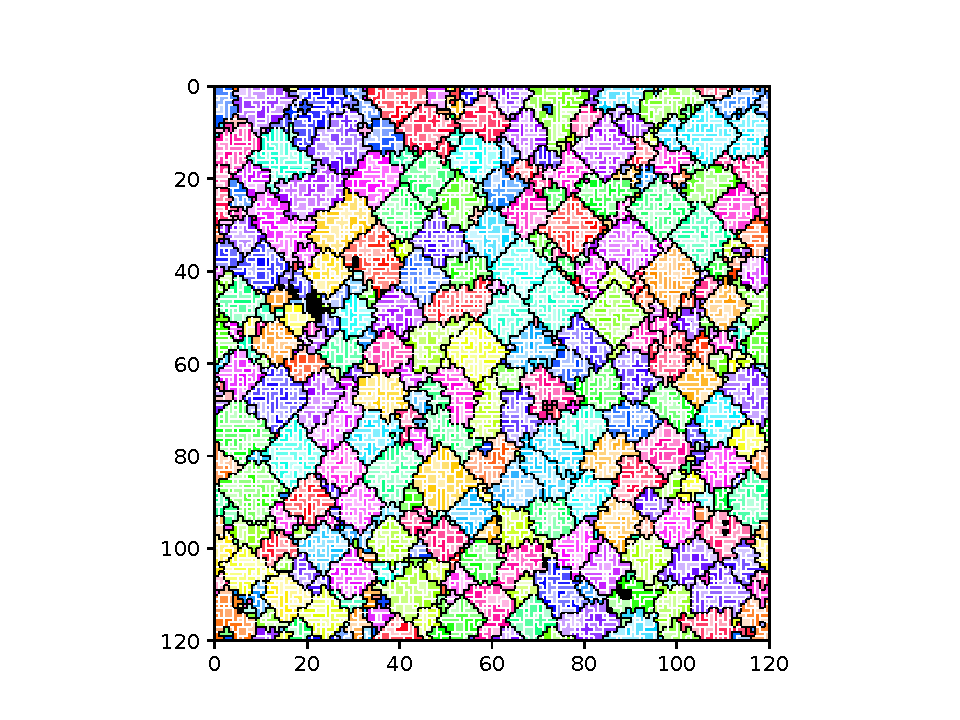
\includegraphics[width=\columnwidth,trim={2.5cm 0.5cm 2.5cm 1cm},clip]{img/ChannelMap_1007_update55520}
  \vspace{-5ex}
  \caption{Update 55520; cell gen. 103}
  \label{fig:ChannelMap_1007_update55520}
\end{subfigure}%
\begin{subfigure}[b]{0.33\columnwidth}
  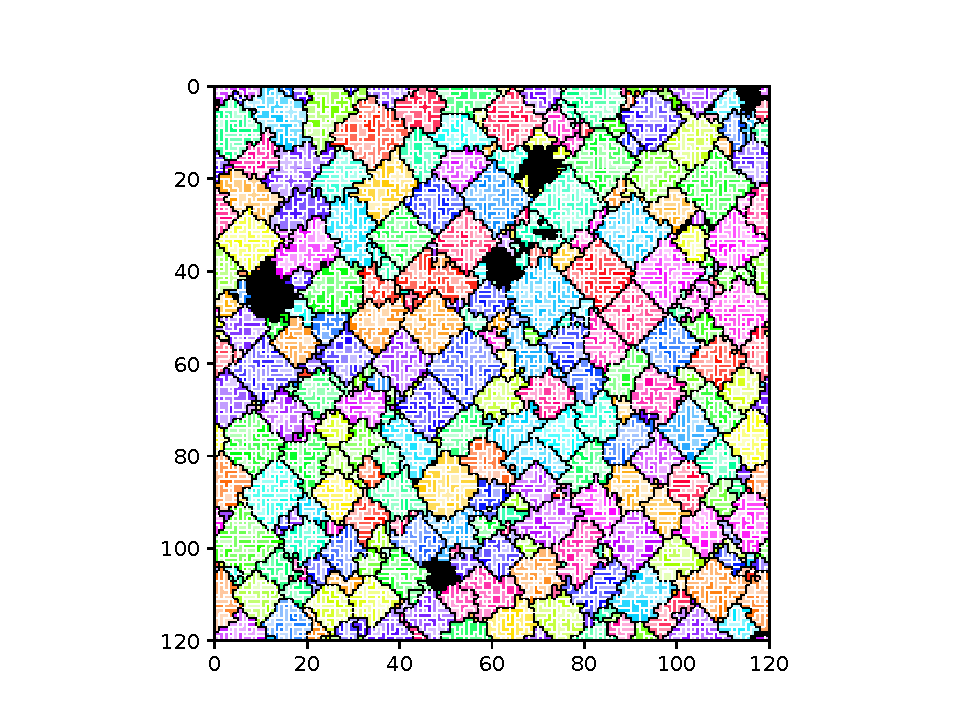
\includegraphics[width=\columnwidth,trim={2.5cm 0.5cm 2.5cm 1cm},clip]{img/ChannelMap_1007_update277600}
  \vspace{-5ex}
  \caption{Update 277600; cell gen. 563}
  \label{fig:ChannelMap_1007_update277600}
\end{subfigure}

\begin{subfigure}[b]{0.33\columnwidth}
  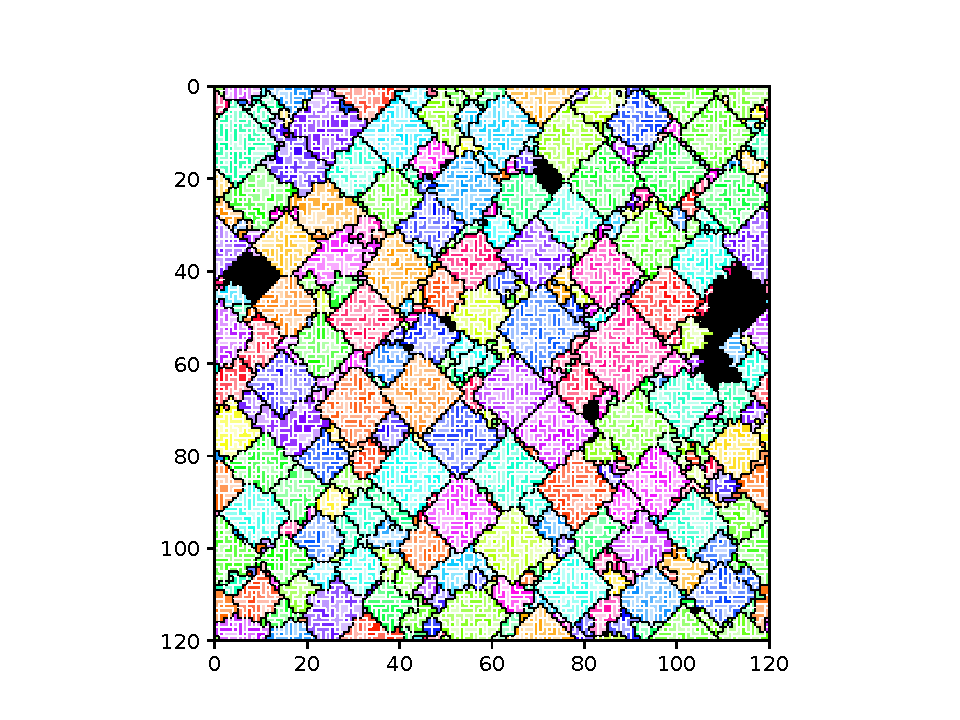
\includegraphics[width=\columnwidth,trim={2.5cm 0.5cm 2.5cm 1cm},clip]{img/ChannelMap_1007_update500000}
  \vspace{-5ex}
  \caption{Update 500000; cell gen. 1072}
  \label{fig:ChannelMap_1007_update500000}
\end{subfigure}%
\begin{subfigure}[b]{0.33\columnwidth}
  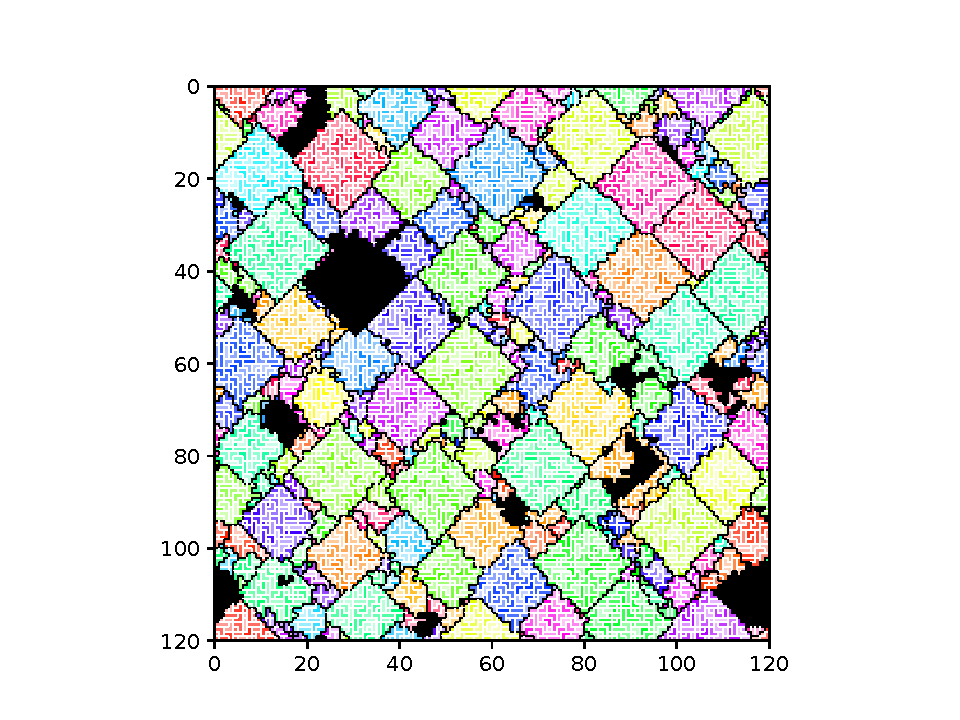
\includegraphics[width=\columnwidth,trim={2.5cm 0.5cm 2.5cm 1cm},clip]{img/ChannelMap_1007_update1000000}
  \vspace{-5ex}
  \caption{Update 1000000; cell gen. 2405}
  \label{fig:ChannelMap_1007_update1000000}
\end{subfigure}%
\begin{subfigure}[b]{0.33\columnwidth}
  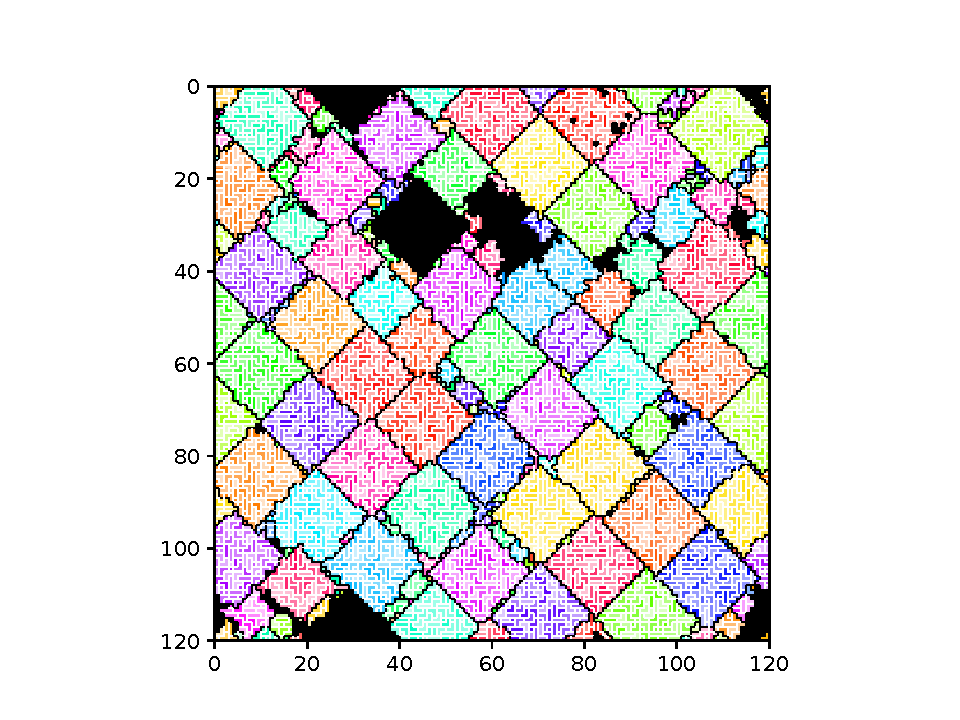
\includegraphics[width=\columnwidth,trim={2.5cm 0.5cm 2.5cm 1cm},clip]{img/ChannelMap_1007_update2000000}
  \vspace{-5ex}
  \caption{Update 2000000; cell gen. 4974}
  \label{fig:ChannelMap_1007_update2000000}
\end{subfigure}

\caption{
Progression of same-channel level-one and level-two signaling networks states in an evolutionary run where level-two resource sharing evolved.
Level-one channels are coded by color saturation and level-two channels are coded by color hue.
A single cell-like organism occupies each grid tile except for black tiles, which are empty.
Level-one same-channel groups appear as uniformly-colored clumps, bounded by a white border.
Level-two same-channel groups appear as same-hue amalgamations of level-one groups, bounded by a black border.
}
\label{fig:grid_progression}
\end{center}
\end{figure*}


A spectrum of resource allocation strategies were observed at the conclusion of different runs of our evolutionary simulation (mean generation 37,168; $s=4,684$).
We interpret these outcomes as ranging between first-level and second-level individuality.
The criteria used to discern these outcomes are described below.
Figure \ref{fig:outcome_grids} shows the level-one and level-two signaling networks at the end of runs where first-, split-, and second-level resource allocation evolved, respectively.
First-level allocators form somewhat irregular level-two amalgamations of diverse level-one networks.
Second-level allocators form highly regular diamond-shaped level-two signaling networks.
Split-allocation individuals exhibit a level-two phenotype of intermediate regularity.
Figure \ref{fig:grid_progression} shows a time series of signaling network snapshots in an evolutionary run where second-level individuality evolved.

Figure \ref{fig:genotypes} describes predominant genotypes observed at the end of our evolutionary simulations.
All evolved genotypes had $A_2$ fixed at $1.0$.
So, reproduction over cells sharing the same level-two channel was universally avoided;
genotypes evolved so that cells declined to reproduce when they were located at the interior of level-two same-channel signaling networks.

However, a variety of resource-caching strategies evolved.
Most-abundant genotypes at the end of nine evolutionary runs exclusively cached resource in organisms' level-one signaling network's pool (i.e., $P_1 = 1.0$).
We observed strategies where resource was primarily, but not entirely, cached in an organism's level-one signaling network pool (i.e., $1.0 > P_1 > P_2$) as the most-abundant genotype at the end of seven evolutionary runs.
In one run, the most-abundant final genotype split resources evenly between an organism's level-one and level-two signaling network pool ($P_1 = P_2 = 0.5$).
Finally, we observed strategies where resource was primarily, but not entirely, cached in an organism's level-two signaling network pool (i.e., $1.0 > P_2 > P_1$) as the most-abundant genotype at the end of 33 evolutionary runs.
We suspect that a trade-off between growth rate and long-term stability contributed to our observation of split resource sharing strategies.
Cell- and level-one resource caching might function something like saving for a rainy day.
Because reproduction over level-two channel-mates was universally avoided, cells and level-one same-channel networks situated at the interior of a larger level-two same-channel network do not expend their resource pools unless the larger level-one same-channel network is damaged, exposing them to directly-adjacent cells of a different level-one channel.
Thus, resource accumulates in cells and level-one pools until the level-one same-channel network comes under stress.
Split allocation might also represent hedging against defection of a second-level channel-mate by via somatic mutation.

Indeed, we did observe selection for apoptosis in the 41 replicates where the dominant genotype employed second-level resource caching.
In these replicates, the average population mean value of $M_{c}$ was 0.68 with standard deviation 0.33, significantly greater than the value $M_{c} = 0.5$ we would expect in the absence of a selective pressure on apoptosis response to mutation ($p < 0.001$, bootstrap test).

\begin{figure}[t]
\begin{center}

\begin{subfigure}[b]{\columnwidth}
  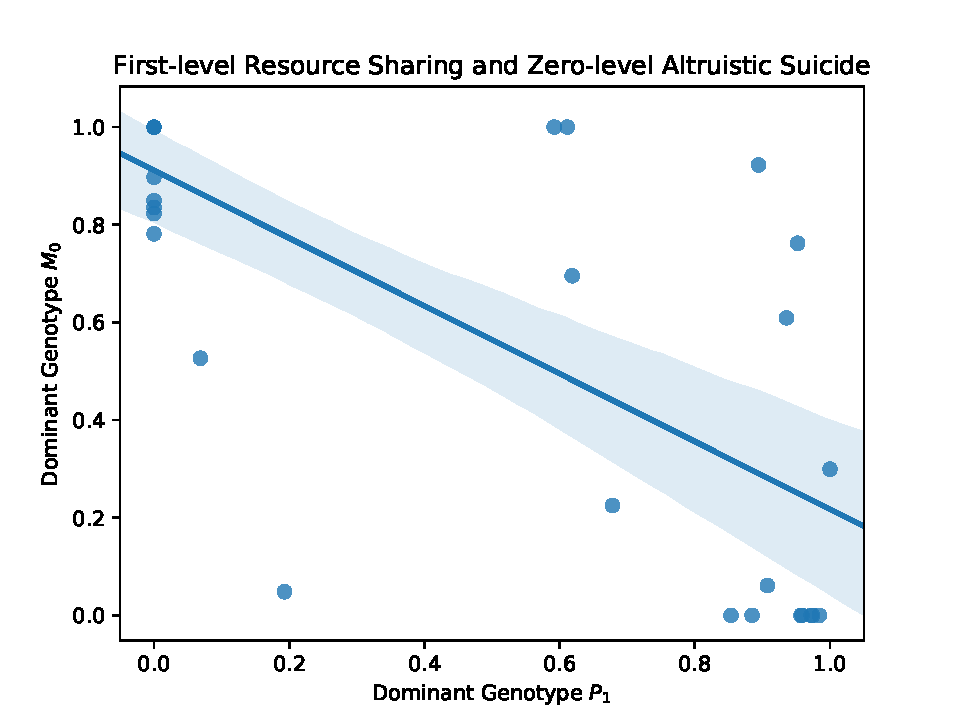
\includegraphics[width=\columnwidth]{img/champion_res_pool1_vs_champion_damage_suicide0}
  \label{fig:champion_res_pool1_vs_champion_damage_suicide0}
\end{subfigure}

\begin{subfigure}[b]{\columnwidth}
  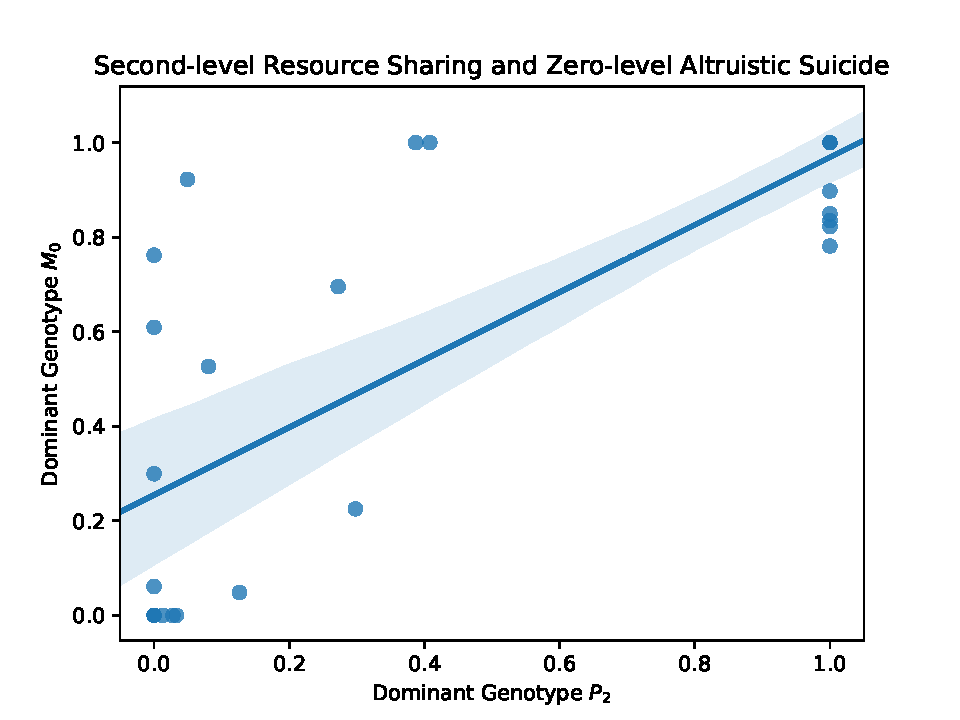
\includegraphics[width=\columnwidth]{img/champion_res_pool2_vs_champion_damage_suicide0}
  \label{fig:champion_res_pool2_vs_champion_damage_suicide0}
\end{subfigure}

\caption{
TODO
}
\label{fig:damage_suicide}
\end{center}
\end{figure}


To assess whether heavy second-level resource allocators, which we characterize as higher-level individuals, were more likely to employ apoptosis to mitigate somatic mutation, we examined the relationship between first- and second-level resource pooling and cellular apoptosis at the conclusion of our 50 replicate evolutionary trials.
We observed a significant negative correlation between dominant genotype $P_1$ and $M_{c}$ ($p < 0.05$; bootstrap test; Figure \ref{fig:champion_res_pool1_vs_champion_damage_suicide0}) and a significant positive correlation between dominant genotype $P_2$ and $M_{c}$ ($p < 0.05$; bootstrap test; Figure \ref{fig:champion_res_pool2_vs_champion_damage_suicide0}).
This result suggests that second-level individuals, in particular, relied on apoptosis to mitigate somatic mutation.

We also assessed whether higher-level individuals provided larger resource endowments to their second-level propagules (offspring sharing neither the level-one nor the level-two channel ID with the parent).
We examined the relationship between first and second-level resource pooling and dominant genotype second-level propagule endowment at the conclusion of our 50 replicate evolutionary trials.
We observed a significant negative correlation between dominant genotype $P_1$ and $E_2$ ($p < 0.05$; bootstrap test) and a significant positive correlation between dominant genotype $P_2$ and $E_2$ ($p <  0.005$; bootstrap test).
Second-level individuals might provide larger endowments to propagules simply due to a greater capacity to collect resource or perhaps because of stronger selection for well-endowed offspring when competing against other second-level individuals.

This result prompts the reverse question: do lower-level individuals provide  larger resource endowments to first-level propagules (offspring that do not share level-one channel ID with the parent but may or may not share level-two channel ID with the parent).
Indeed, we observed a significant positive correlation between first-level resource sharing and first-level endowment ($p < 0.0001$; bootstrap test) and a significant negative correlation between second-level resource sharing and first-level endowment ($p < 0.0001$; bootstrap test).
Cells that pool resource with their smaller level-one same-channel group tend to invest more heavily into the direct offshoots of their level-one same-channel group than cells that pool resource with their larger level-two same-channel group.
This observation suggests that, although cells do not directly displace their level-one channel-mates, competitive dynamics between may be at play more conservative

\subsection{Competition Experiments}

\begin{figure*}%[!htbp]
\begin{center}


\begin{subfigure}[b]{0.9\columnwidth}
  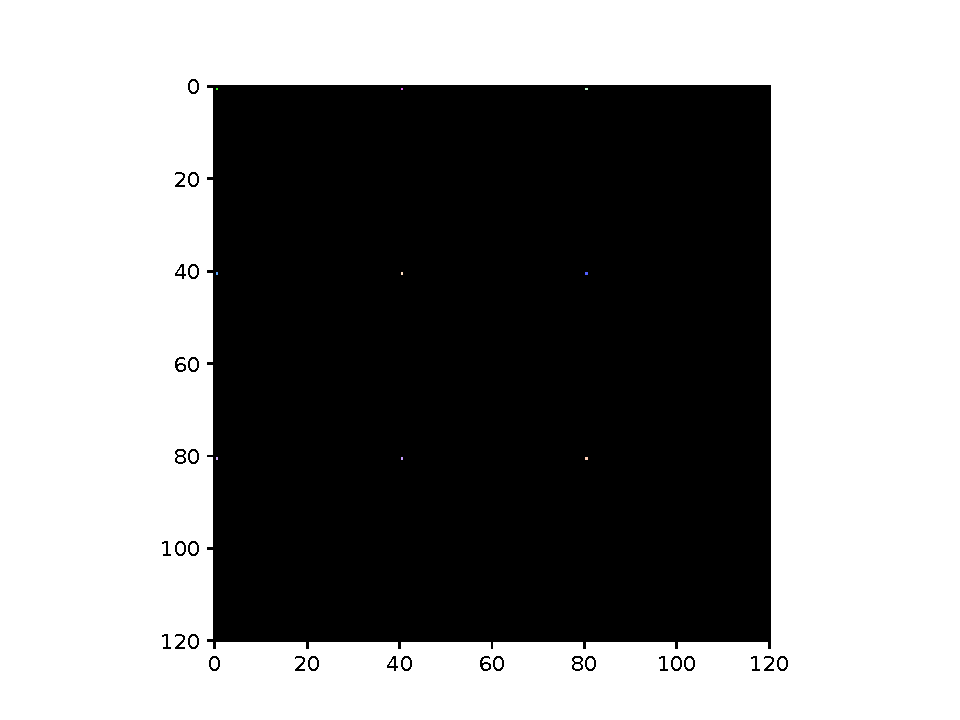
\includegraphics[width=\columnwidth,trim={2.5cm 0.5cm 2.5cm 1cm},clip]{img/ChannelMap_1030_update0}
  \caption{Update 0; cell gen. 0}
  \label{fig:ChannelMap_1030_update0}
\end{subfigure}%
\begin{subfigure}[b]{0.9\columnwidth}
  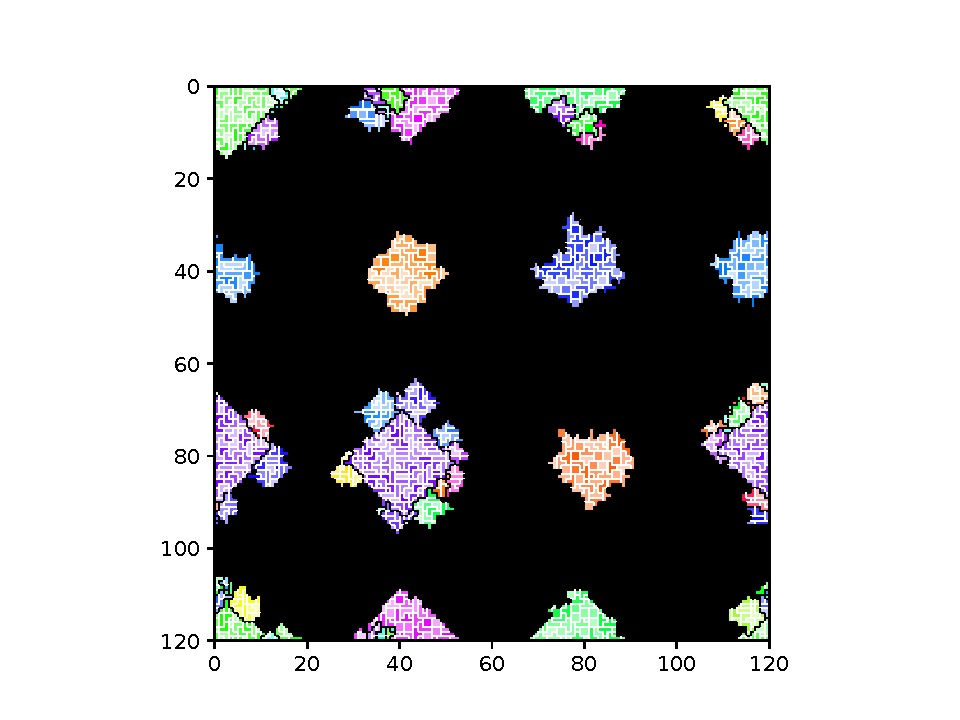
\includegraphics[width=\columnwidth,trim={2.5cm 0.5cm 2.5cm 1cm},clip]{img/ChannelMap_1030_update5552}
  \caption{Update 5552; cell gen. 4}
  \label{fig:ChannelMap_1030_update55520}
\end{subfigure}

\begin{subfigure}[b]{0.9\columnwidth}
  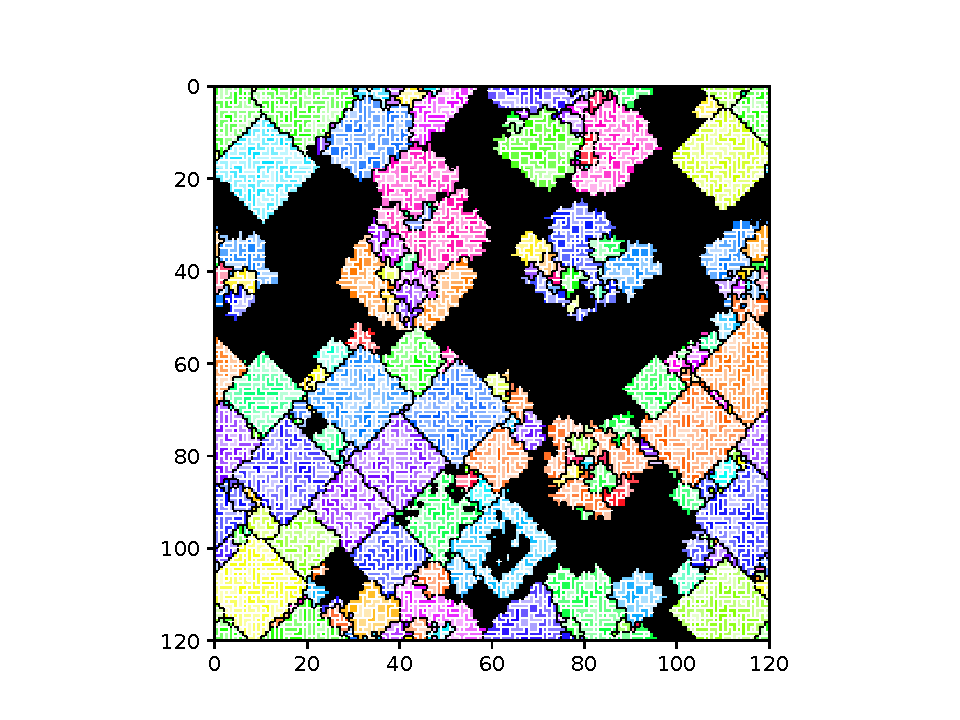
\includegraphics[width=\columnwidth,trim={2.5cm 0.5cm 2.5cm 1cm},clip]{img/ChannelMap_1030_update11104}
  \caption{Update 1104; cell gen. 9}
  \label{fig:ChannelMap_1030_update277600}
\end{subfigure}%
\begin{subfigure}[b]{0.9\columnwidth}
  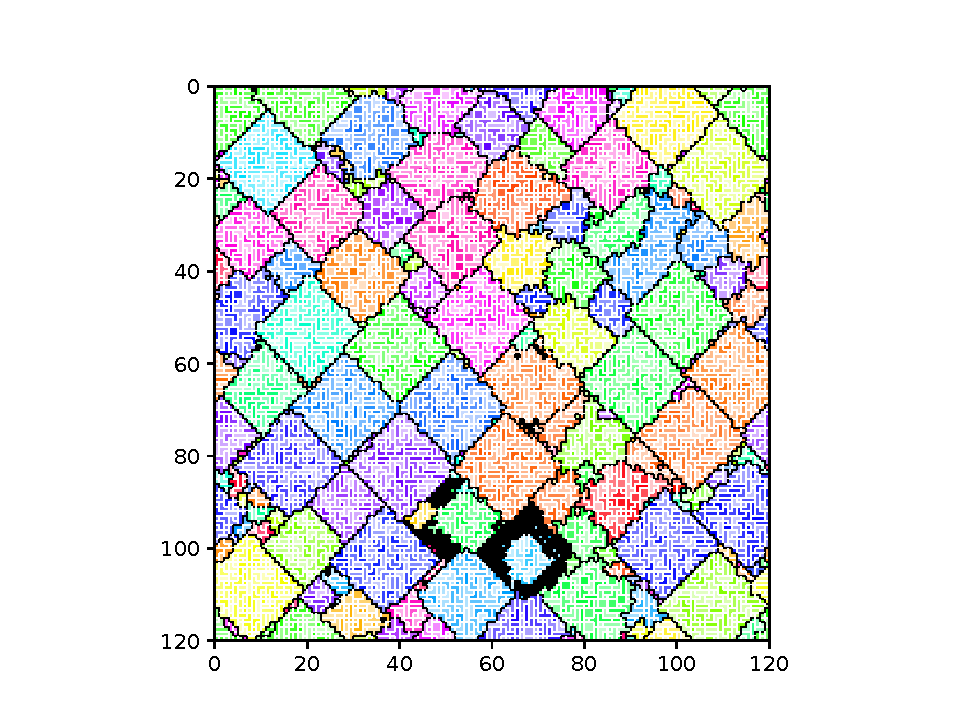
\includegraphics[width=\columnwidth,trim={2.5cm 0.5cm 2.5cm 1cm},clip]{img/ChannelMap_1030_update22208}
  \caption{Update 22208; cell gen. 32}
  \label{fig:ChannelMap_1030_update22208}
\end{subfigure}

\begin{subfigure}[b]{0.9\columnwidth}
  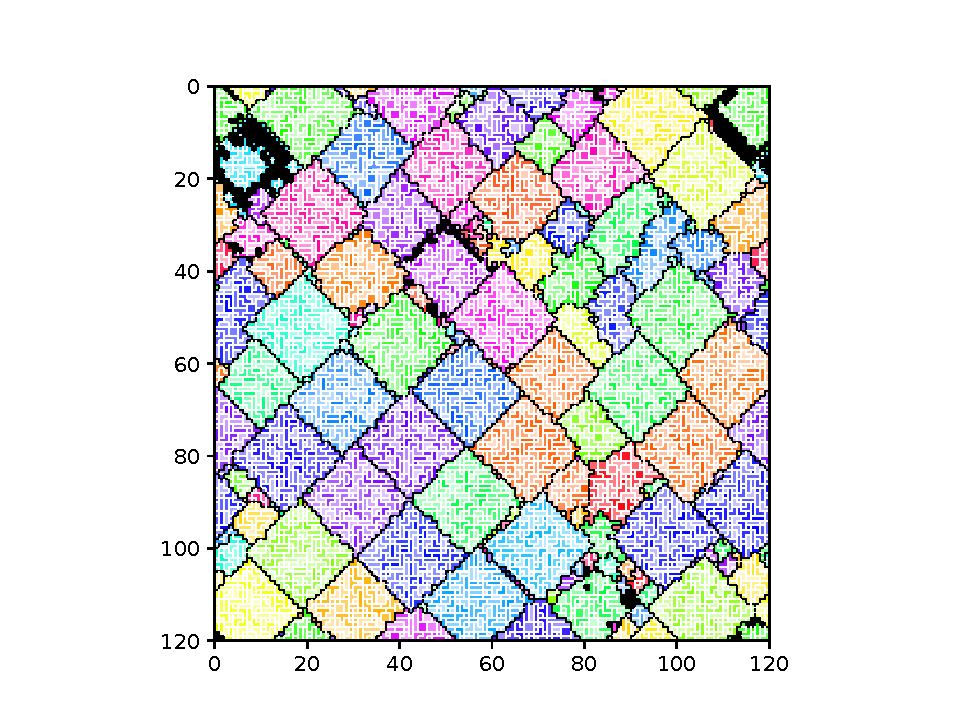
\includegraphics[width=\columnwidth,trim={2.5cm 0.5cm 2.5cm 1cm},clip]{img/ChannelMap_1030_update55520}
  \caption{Update 55520; cell gen. 107}
  \label{fig:ChannelMap_1030_update1000000}
\end{subfigure}%
\begin{subfigure}[b]{0.9\columnwidth}
  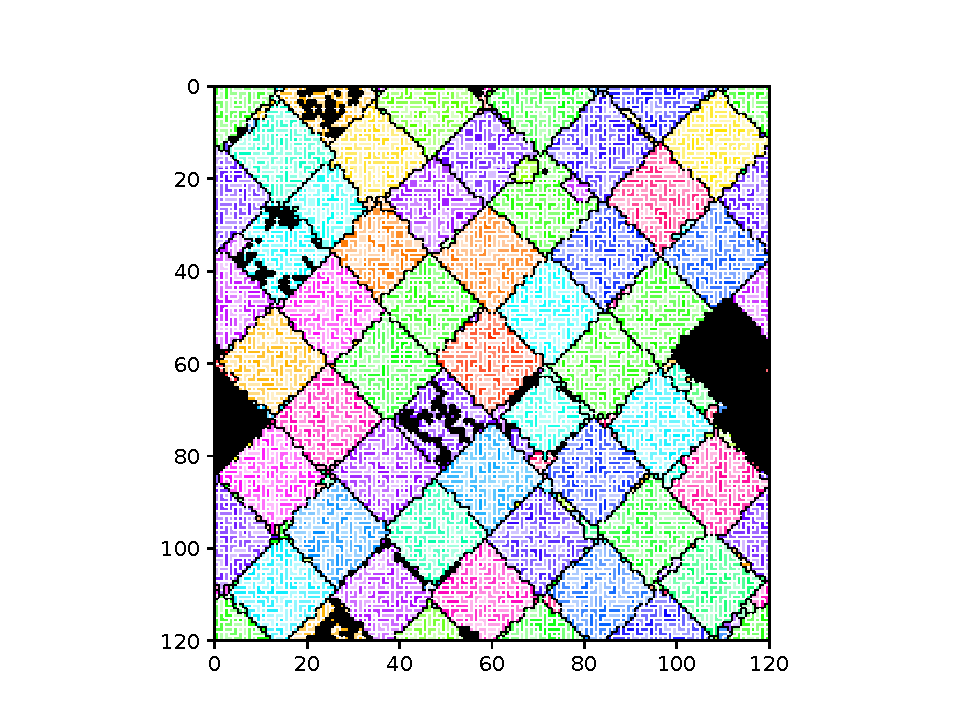
\includegraphics[width=\columnwidth,trim={2.5cm 0.5cm 2.5cm 1cm},clip]{img/ChannelMap_1030_update1500000}
  \caption{Update 1500000; cell gen. 3511}
  \label{fig:ChannelMap_1030_update1500000}
\end{subfigure}
\caption{
Progression of of same-channel level-one and level-two signaling networks states in a competition run.
We seeded the grid with three copies of each of three champion genotypes from evolutionary trials.
Then, with mutation disabled to prevent further evolution, the genotypes competed.
Level-one channels are coded by color saturation and level-two channels are coded by color hue.
A single cell-like organism occupies each grid tile except for black tiles, which are empty.
}
\label{fig:eco_progression}
\end{center}
\end{figure*}


Next, we wanted to compare first-, second-, and split-level allocators to determine which genotype was the most fit.
We ran competition experiments between dominant genotypes from evolutionary runs representative of each of these strategies.
To represent first-level allocators, we selected randomly from the nine pure first-level allocator dominant genotypes we observed.
To represent the split-level allocators, we selected the single dominant genotype where resource was partitioned exactly evenly between first- and second-level channel pools.
To represent second-level allocators, we selected the dominant genotype with the largest second-level allocation proportion.
Figure \ref{fig:genotypes} enumerates the three representative genotypes used.
Figure \ref{fig:eco_progression} shows a time series of signaling network snapshots in an competition experiment run.
Colonies of each genotype can be seen to grow from each seed and then clash, ultimately yielding a population dominated by second-level allocators.

Indeed, the second-level resource caching strategy became most abundant in all 50 trials.
Across the 50 replicates, the second-level resource caching strategy constituted $90.2 \%$, with standard deviation $3.8 \%$, of the competing population of cells.
In the absence of mutation, second-level individuals tend to exhibit greater fitness than evenly-split-allocation and first-level individuals ($p < 0.0001$; two-tailed exact test).


\begin{figure}[t]
\begin{center}

\begin{subfigure}[b]{\columnwidth}
  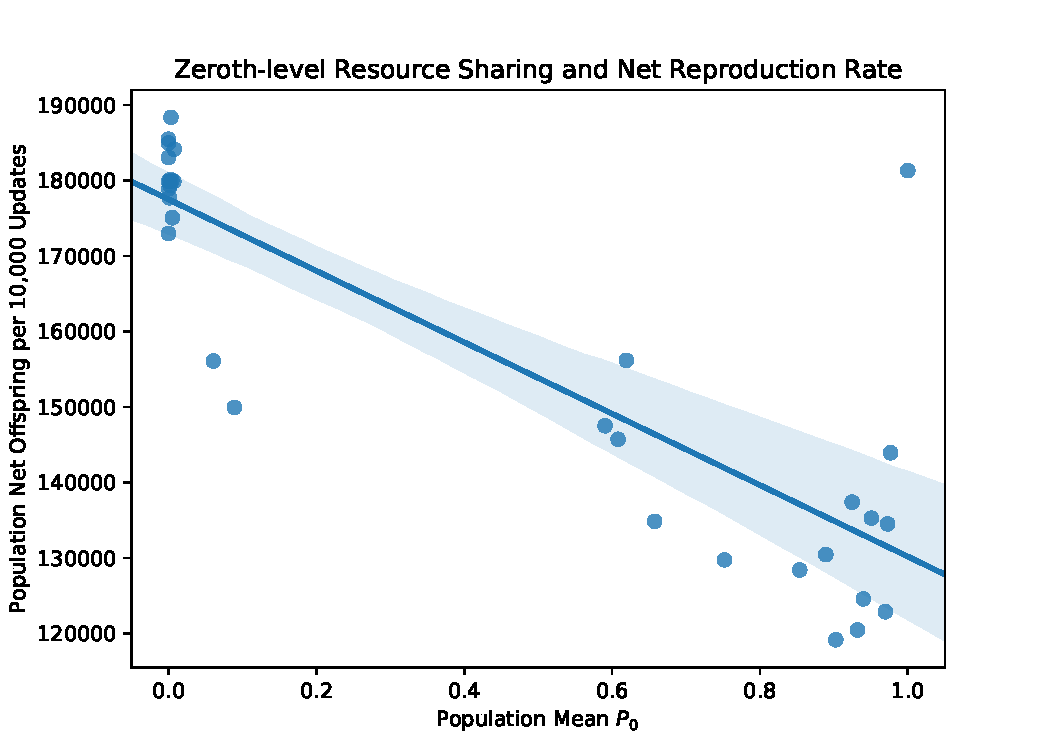
\includegraphics[width=\columnwidth]{img/mean_res_pool1_vs_net_reproduction}
  \caption{
  Correlation plot of population mean $P_1$ and population net reproduction rate.
  }
  \label{fig:mean_res_pool1_vs_net_reproduction}
\end{subfigure}

\begin{subfigure}[b]{\columnwidth}
  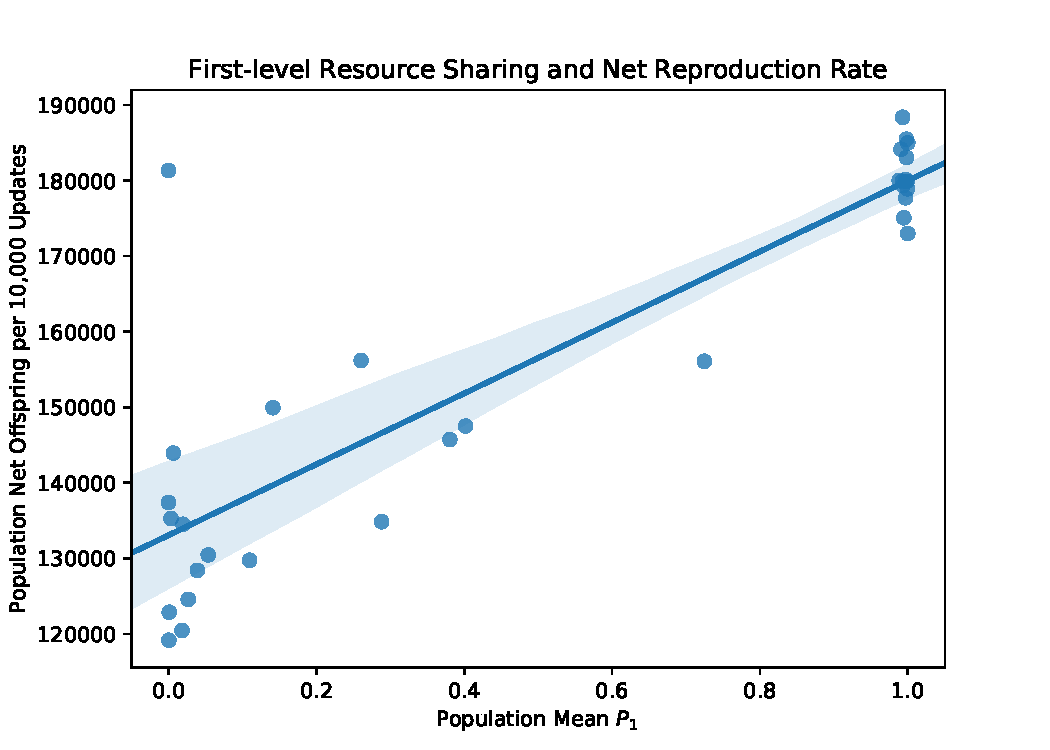
\includegraphics[width=\columnwidth]{img/mean_res_pool2_vs_net_reproduction}
  \caption{
  Correlation plot of population mean $P_2$ and population net reproduction rate.
  }
  \label{fig:mean_res_pool2_vs_net_reproduction}
\end{subfigure}

\caption{
Plot of population mean resource caching strategies and population net reproduction rate.
}
\label{fig:net_reproduction}
\end{center}
\end{figure}


In competition experiments, however, higher-level individuals likely benefited from elimination of somatic mutation.
To assess the relative fitness of first- and second-level individuals without mutation disabled, we examined the relationship between first- and second-level resource pooling and the rate of cellular reproduction at the end of each of the 50 replicate evolutionary trials performed.
We observed a significant negative correlation between mean $P_1$ and cellular reproduction rate ($p < 0.0001$; bootstrap test; Figure \ref{fig:mean_res_pool1_vs_net_reproduction}) and a significant positive correlation between mean $P_2$ and cellular reproduction rate ($p < 0.0001$; bootstrap test; Figure \ref{fig:mean_res_pool2_vs_net_reproduction}).
This result suggests that second-level individuals tend to collect resource more effectively than evenly-split-allocation and first-level individuals.

\subsection{Control Evolutionary Experiments}

\begin{figure}%[!htbp]
\begin{center}
\thinmuskip=-2mu
\thickmuskip=-2mu
\nulldelimiterspace=-1pt
\scriptspace=0pt

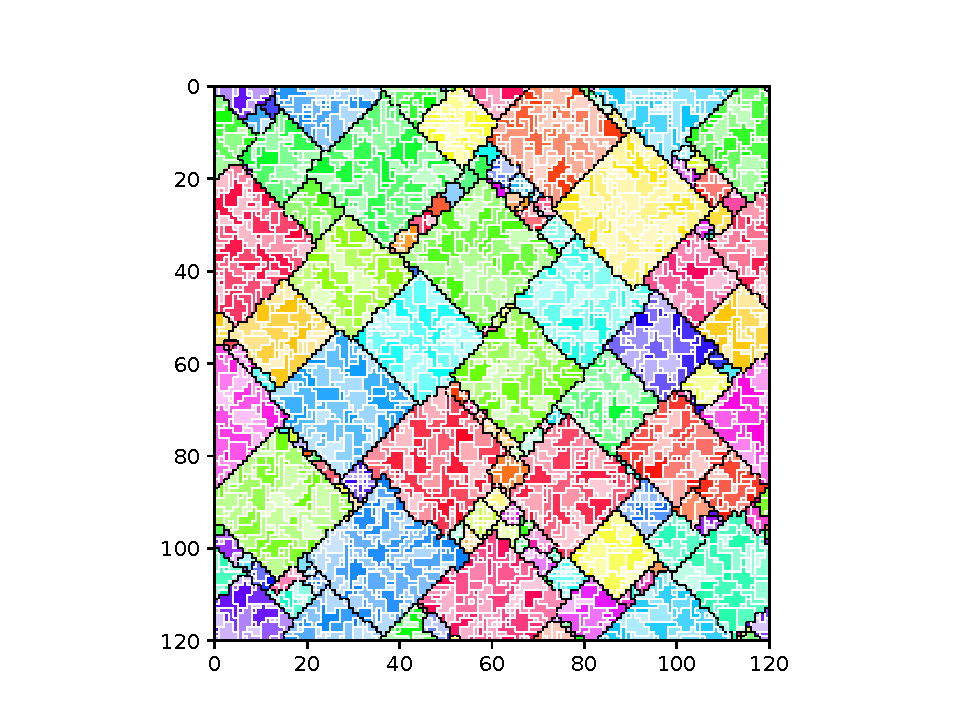
\includegraphics[width=\columnwidth,trim={2.5cm 0.5cm 2.5cm 1cm},clip]{img/ChannelMap_1018_update249840}

\caption{
End state of same-channel signaling networks in a randomly chosen replicate from the control treatment.
Update 249840, cell generation 5384.
Level-one channels are coded by color saturation and level-two channels are coded by color hue.
A single cell-like organism occupies each grid tile except for black tiles, which are empty.
}
\label{fig:outcome_control}
\end{center}
\end{figure}


Under control conditions, we observed strong selection for high-level resource caching.
At update 200,000, the average population mean of $P_2$ was 0.96 with standard deviation 0.08.
For comparison, under the standard treatment the average population mean of $P_2$ was 0.54 with standard deviation 0.11 at a time-point matched by absolute elapsed update count and 0.55 with standard deviation 0.22 at a time-point matched by approximate elapsed cellular generations\footnote{This statistic is affected by missing datafile entries for two standard treatment replicates due to server instability.} (Figure \ref{fig:genotypes}).
We also observed strong selection against direct reproductive competition between channel-mates at update 200,000; all evolved genotypes completely avoided reproducing over level-two channel-mates.

The emergence of resource-sharing and competition avoidance under control conditions suggest kin recognition alone can prompt some aspects of higher-level individuality.
However, we observed selection against the apoptosis response to mutation, $M_{c}$, under control conditions.
Across 50 replicates of the control treatment, the average population mean value of $M_{c}$ was 0.20 with standard deviation 0.23 --- significantly less than the value $M_{c} = 0.5$ expected without selective pressure against apoptosis response to mutation ($p < 0.0001$, bootstrap test).
Indeed, population mean $M_{c}$ for control runs was also significantly reduced compared to the standard treatment at time-points matched by absolute elapsed update count ($p < 0.0001$; two-tailed t test) and by approximate elapsed cellular generations ($p < 0.01$; two-tailed t test)
\footnote{This comparison is affected by missing datafile entries for two standard treatment replicates due to server instability.}.
Perhaps under control conditions, the apoptosis response to mutation is disfavored because kin groups stand to lose less from mutant members (i.e., the resource penalty for excessive same-channel network expansion is absent).
It appears that, at least in our system, kin recognition alone does not suffice to prompt full-fledged fraternal transitions in individuality.

In the absence of resource penalties for erroneous activation under control conditions, we also observed the evolution of larger level-one same-channel groups.
Compared to the standard treatment, control runs exhibited greater mean level-two same-channel caps $C_2$ at time-points matched by absolute elapsed update count ($p < 0.0001$; two-tailed t test) and approximate elapsed cellular generations ($p < 0.0001$; two-tailed t test)\footnote{This comparison is affected by missing datafile entries for two standard treatment replicates due to server instability.}.
Even at the 20 million updates mark, when evolution had elapsed around ten times as many cellular generations in the standard treatment compared to the control treatment at update 200,000, mean level-two same-channel caps $C_2$ reached only 262.9 with standard deviation 72.2 under the control treatment.
This is significantly($p < 0.0001$; two-tailed t test).
Figure \ref{fig:outcome_control}, which visualizes the comparatively large same-channel level two groups present at the end of a control run.
